\documentclass[11pt,italian]{article}
\usepackage[T1]{fontenc}
\usepackage[utf8]{inputenc} %utf8 % lettere accentate da tastiera
\usepackage[italian]{babel} % lingua del documento
\usepackage{blindtext}
\usepackage{enumitem}
\usepackage{graphicx}
\usepackage{float}
\usepackage{xcolor}   % for \textcolor
\usepackage[font=small,labelfont=bf,skip=3pt]{caption}
\setlength{\belowcaptionskip}{-10pt}
\usepackage{listings}
\lstset{
    basicstyle=\small\ttfamily,
    columns=fullflexible,
    frame=single,
    breaklines=true,
    postbreak=\mbox{\textcolor{red}{$\hookrightarrow$}\space},
    tabsize=4, % tab space width
    showstringspaces=false, % don't mark spaces in strings
    numbers=left, % display line numbers on the left
    commentstyle=\color[HTML]{a0a1a7}, % comment color
    keywordstyle=\color[HTML]{40a3f5}, % keyword color
    stringstyle=\color{red}, % string color,
    emphstyle={\color[HTML]{40a3f5}}
}
\usepackage{hyperref}
\usepackage{cleveref}
\hypersetup{
    colorlinks = true,
    linkbordercolor = {white},
    urlcolor = blue
}
\usepackage{graphicx}
\graphicspath{ {./images/} }

% Italian syntax spacing
\frenchspacing

% Line height
\renewcommand{\baselinestretch}{1.15}

% Use lstinline as item in description
\makeatletter
\newcommand*{\lstitem}[1][]{%
  \setbox0\hbox\bgroup
    \patchcmd{\lst@InlineM}{\@empty}{\@empty\egroup\item[\usebox0]\leavevmode\ignorespaces}{}{}%
    \lstinline[#1]%
}
\makeatother

\title{
    Metodi del Calcoli Scientifico \\
    \normalsize Implementazione della funzione DCT2 e confronto con \lstinline{scipy} \\
	\normalsize Progetto 2 / Parte 1
}

\date{A.A.: 2019/2020}

\author{
	\normalsize
	\textsc{Edoardo Silva 816560} \\
	\normalsize
	\textsc{Bryan Zhigui 816335} \\
	\normalsize
	\textsc{Davide Marchetti 815990}
}

\begin{document}
\maketitle

\section*{Abstract}
Si vuole avere un confronto dei tempi d’esecuzione della DCT2 della libreria scelta con la nostra implementazione elaborando matrici quadrate generate casualmente.
I risultati ottenuti saranno riportati graficamente in un grafico a scala semi-logaritmica.

\newpage
\section{Librerie}
\subsubsection*{Numpy}
Libreria open source che contiene diverse funzioni e metodi utili per il calcolo scientifico. In particolar modo per il calcolo vettoriale e di matrici multidimensionali in maniera efficiente e veloce.

\subsubsection*{Scipy}
Libreria open source che utilizza le funzionalità di Numpy per fornire un pacchetto di calcolo scientifico General-purpose. In particolare, in questo progetto si utilizza l'estensione \textbf{Fast Fourier Transform} (\lstinline{fftpack}) per lavorare con la \lstinline{DCT monodimensionale} e \lstinline{multidimensionale}(\textbf{DCT2}).

\subsubsection*{Pandas}
Fornisce una serie di strumenti per elaborare e manipolare dati in formato tabellare (\lstinline{DataFrame}) interfacciandosi con le strutture dati native in Python.

\subsubsection*{Matplotlib}
Permette di generazione grafici di svariate tipologie.
Il modulo \lstinline{pyplot} fa da interfaccia alle API più a basso livello per la generazione di codice.

\subsubsection*{Seaborn}
Utilizzato principalmente per la creazione di grafici statistici. Agisce come un wrapper per la libreria \lstinline{matplotlib} semplificandone alcune funzionalità per la creazione di grafici complessi.

\subsection{Implementazione della DCT in Scipy}
\label{section:scipy-fft}
Dalla documentazione del modulo \lstinline{scipy.fftpack}\footnote{\url{http://wwwens.aero.jussieu.fr/lefrere/master/SPE/docs-python/scipy-doc/generated/scipy.fftpack.dct.html}} viene referenziato un documento che descrive dal punto di vista matematico l'implementazione della DCTN nella libreria.

\noindent
L'abstract del paper \textit{"A fast cosine transform in one and two dimensions"} di \textit{Makhoul, J. (Feb. 1980)}\footnote{\url{https://ieeexplore.ieee.org/document/1163351}} riporta:
\begin{quote}
    The discrete cosine transform (DCT) of an $N$-point real signal is derived by taking the discrete Fourier transform (DFT) of a $2N$-point even extension of the signal.
    It is shown that the same result may be obtained using only an $N$-point DFT of a reordered version of the original signal, with a resulting saving of 1/2.
    If the fast Fourier transform (FFT) is used to compute the DFT, the result is a fast cosine transform (FCT) that can be computed using on the order of $N log_2(N)$ real multiplications.
    The method is then extended to two dimensions, with a saving of 1/4 over the traditional method that uses the DFT.
\end{quote}

\noindent
Si presume quindi, di notare notevoli miglioramenti rispetto all'applicazione della DCT da noi implementata.

\newpage
\section{Implementazione della DCT/DCTN}
\subsection{DCT}
La funzione $\mathit{DCT}$ prende in input un vettore $V$ di dimensione $N$ ed esegue le seguenti operazioni:
\begin{enumerate}
    \item Viene pre-allocato un vettore $C$ di dimensione $N$ con componenti tutte pari a zero.
    \item Per ogni elemento del vettore $V$ di input:
    \begin{enumerate}
        \item Viene calcolato il coefficiente $C[k]$ nella base $w_k$ del valore $V[i]$
        \item Questo viene scalato per un certo valore $\alpha_k$
    \end{enumerate}
    \item Il vettore risultante $C$ viene ritornato come vettore in output
\end{enumerate}

\begin{lstlisting}[language=python,emph={math,np},caption=Implementazione della DCT monodimensionale]
def dct(V):
    N = len(V)
    c = np.zeros(N)
    for k in range(N):
        s = 0

        for i in range(N):
            s += V[i] * np.cos(k * np.pi * ((2*i+1) / (2*N)))

        alpha = 1 / math.sqrt(N) if k == 0 else math.sqrt(2 / N)
        c[k] = alpha * s

    return c
\end{lstlisting}

\subsection{DCT2}
\label{section:dct2}
La implementazione della DCT2 sfrutta l'applicazione della DCT monodimensionale su colonne e righe per ottenere la scomposizione corretta.

Nell'algoritmo, l'input risulta essere una matrice quadrata $\mathit{Mat}$ di dimensione $N\times N$. Inoltre, viene definita una matrice intermedia $C$ inizializzata a zero la quale sarà elaborata a partire dalla matrice in input per ottenere l'applicazione corretta della DCT2.

Inizialmente si effettua la $\mathit{DCT}$ monodimensionale prima sui vettori colonna della matrice originale salvando i risultati ottenuti nella matrice $C$ e, successivamente, sui vettori riga della stessa appena popolati.

\begin{lstlisting}[language=python,emph={math,np},caption=Implementazione della DCT multidimensionale (DCT2)]
def dct2(Mat):
    N, M = Mat.shape

    C = np.zeros((N, M), dtype='float')
    for j in range(M):
        C[:, j] = dct(Mat[:, j])


    for i in range(N):
        C[i, :] = dct(C[i, :])

    return C
\end{lstlisting}

\newpage
\section{Esecuzione}
Il fulcro del programma consiste in una funzione (listato \ref{code:main-function}) che accetta in input tre parametri:
\begin{description}
    \lstitem{offset:} da che dimensione generare le matrici
    \lstitem{how_many:} numero di matrici da generare e confrontare
    \lstitem{step:} di quanto incrementare la dimensione della matrice ad ogni iterazione
\end{description}

\noindent
La funzione esegue quindi i seguenti step:
\begin{enumerate}
    \item Genera una matrice quadrata \lstinline{problem} di dimensione \lstinline{size} con valori randomici in un range $[0,255]$.
    \item Applica la \lstinline{DCTN} di tipo 2 con norma ortogonale tenendo traccia del tempo di esecuzione
    \item Salva dimensione e tempo impiegato per l'esecuzione \lstinline{scipy} in un vettore \lstinline{matrices}
    \item Applica la \lstinline{DCT2} implementata come descritto nella \cref{section:dct2} tenendo traccia del tempo di esecuzione.
    \item Memorizza dimensione e tempo di esecuzione dell'implementazione manuale nello stesso vettore.
\end{enumerate}
\noindent
Una volta terminato il ciclo, il vettore \lstinline{matrices} conterrà $2\times$\lstinline{how_many} elementi: i risultati da visualizzare su grafico per il confronto.

\newpage
\begin{lstlisting}[language=python,emph={math,np},label=code:main-function,caption=Funzione per il confronto tra implementazioni]
def performance_test(offset, how_many, step=1):
    matrices = []

    for index in range(0, how_many*step, step):
        size = index + offset
        problem = np.random.randint(0, 255, size=(size, size))

        tic = time.perf_counter()
        dctn(problem, type=2, norm='ortho')
        toc = time.perf_counter()

        matrices.append({
            'size': size,
            'duration': float(toc - tic),
            'type': 'scipy'
        })

        tic = time.perf_counter()
        custom_dct.dct2(problem)
        toc = time.perf_counter()

        matrices.append({
            'size': size,
            'duration': float(toc - tic),
            'type': 'implemented'
        })

    return matrices
\end{lstlisting}

\newpage
\section{Risultati}
\label{section:results}
La \cref{fig:execution-time} riporta il tempo di esecuzione posto sulle ordinate e la dimensione della matrice generata sulle ascisse.

Quest'ultima copre un range da $10$ a $150$ ad incrementi di $5$ unità tra una matrice e la successiva.

\begin{figure}[H]
    \makebox[\textwidth][c]{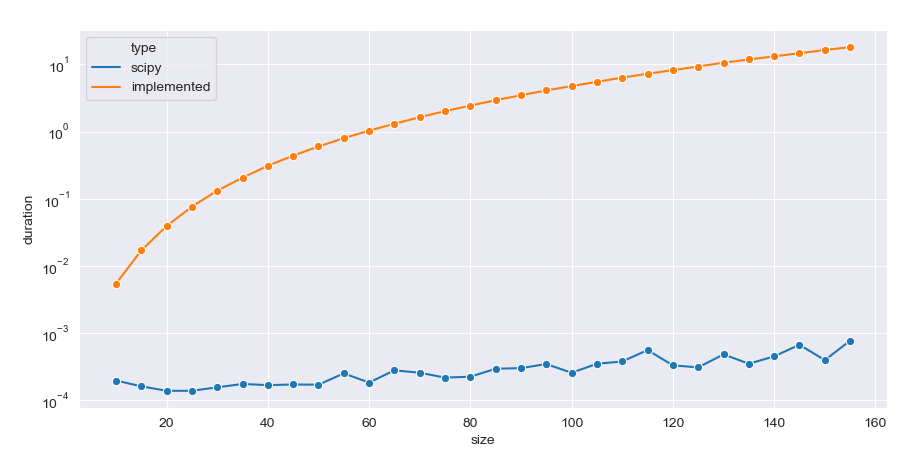
\includegraphics[width=1.3\linewidth]{results.png}}
    \caption{Confronto tra la DCT2 in \lstinline{scipy} e la nostra implementazione}
    \label{fig:execution-time}
\end{figure}

\newpage
\section{Conclusioni}
L'implementazione proposta dal documento citato nella \cref{section:scipy-fft} risulta quindi confermata dal confronto riportato in \cref{fig:execution-time} ed è sempre più evidente al crescere della dimensione della matrice da elaborare.

Dall'analisi grafica possiamo notare che la \lstinline{DCT2} implementata manualmente segue un andamento riconducibile ad un $O(N^3)$, invece l'implementazione utilizzata in \lstinline{scipy} delinea un andamento altalenante tra $O(NlogN)$) e $O(N^2)$.

Naturalmente, ci si aspettava che la nostra implementazione risultasse decisamente più lenta dell'implementazione FFT, tuttavia il risultato ottenuto in termini numerici risulta equiparabile con entrambi i metodi.
\end{document}
